% Multiple Choice Question 2

\begin{center}
    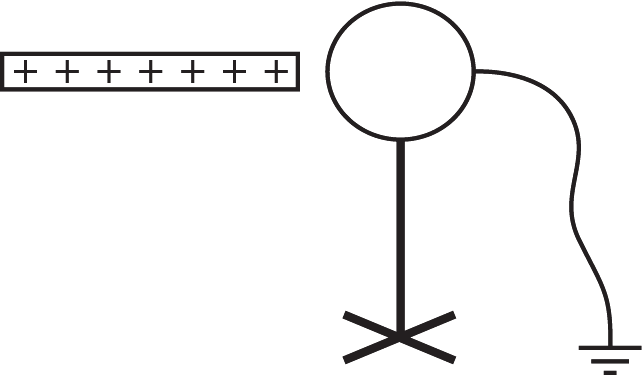
\includegraphics[scale=0.25]{images/img-002-000.png}
\end{center}

\begin{questions}
\setcounter{question}{1}

\question
A grounded spherical conductor is on an insulating stand. A positively charged rod is brought close to the sphere but does not touch the sphere, as shown above. The rod is moved far away and then the grounding wire is removed. Which of the following describes the resulting charge on the sphere?

\begin{choices}
    \choice Positive
    \choice Negative
    \choice No net charge, but it is polarized with positive charges on the left side of the sphere
    \choice No net charge, but it is polarized with negative charges on the left side of the sphere
    \choice No net charge and no polarization
\end{choices}

\end{questions}
